%Test-Driven Development
%- O que é?
%  --> Feedback constante, rápido e barato.
%- Prática de testes ou design?
%  --> diferenca do feedback de uma prática de teste para uma prática de design
%- Feedback no design
%- Design emergente
%- Mercado atual

%% ------------------------------------------------------------------------- %%
\chapter{Test-Driven Development}
\label{cap:tdd}

Métodos ágeis de desenvolvimento de software focam sempre em constante
feedback, seja ele da equipe em relação ao cliente, ou da equipe em relação a
qualidade (interna e externa) do código produzido. Por esse motivo, muitas das
práticas sugeridas por esses métodos tentam aumentar o quantidade e a qualidade
desse feedback; a ideia da programação pareada, por exemplo, é dar retorno
sobre o código alguns segundos após ele ter sido escrito.

Test-Driven Development (TDD), popularizada pelo Kent Beck através de seu livro
\textit{TDD: By Example} em 2001 \cite{TDDByExample}, é mais uma das práticas
ágeis onde o foco é dar feedback. TDD tem grande importância durante o ciclo de
desenvolvimento já que, conforme sugerido pelas práticas ágeis, o design de um
software deve emergir a medida que o software cresce. E, para responder
rapidamente a essas alterações, é necessário um constante feedback sobre a
qualidade interna e externa do código.

A velocidade que a prática dá retorno ao desenvolvedor possibilita que o mesmo
tome decisões de design sobre o código enquanto o custo de mudança ainda é
baixo. Segundo Vanderburg, TDD dá feedback em questão de minutos, e sua
velocidade só é inferior a da programação pareada. O gráfico pode ser visto na
figura \ref{fig:agile-feedback}.

% TODO: traduzir figura do meu gdocs
\begin{figure}
  \centering
  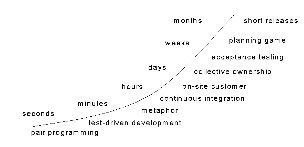
\includegraphics[scale=1]{agile-feedback}
  \caption{Práticas de XP e Tempo de Feedback}
  \label{fig:agile-feedback}
\end{figure}

Em uma definição mais formal, TDD é a arte de produzir testes automatizados para
código de produção, usando esse processo para guiar o design e a programação.
Para cada pequeno pedaço de funcionalidade, o desenvolvedor deve primeiro
escrever um teste que especifique e valide o que o código irá fazer. O
programador então produz somente o código necessário para fazer esse teste
passar. Então ele refatora (simplifica e clareia) tanto o código de produção
quanto o código de testes \cite{agilealliance-tdd} \cite{tdd-taxonomy}.

% TODO: citar
Na opinião de muitos autores conhecidos, como Kent Beck, Martin Fowler e Robert
Martin, essa mudança na ordem do ciclo de desenvolvimento tradicional, apesar de
simples, agrega diversos benefícios ao código produzido: simplicidade, foco,
melhor design, entre outras.

% TODO: citar tddesign
Apesar da criação de testes ser algo intríseco ao processo, TDD não é visto como
uma prática fundamentalmente de testes, mas sim uma prática que auxilia o
desenvolvedor a desenhar classes mais flexíveis, mais coesas e menos acopladas.
Por esse motivo, muitos se referem a TDD como \textit{Test-Driven Design}, ou
seja, design guiado pelos testes.

Muitos autores afirmam que TDD é na verdade uma prática de design
\cite{tdd-taxonomy} \cite{aim-fire}, e citam sempre a famosa frase do Ward
Cunningham, um dos pioneiros da Programação Extrema: \textit{Test-First
programming is not a testing technique} que, em uma tradução livre, significa
\textit{Programação Teste Primeiro (Test-First Programming) não é uma prática
de testes}.

\section{Definições incompletas}

Apesar do foco da prática em design, é possível encontrar muitas definições que
não levam isso em conta. Algumas delas levam em consideração apenas a ideia da
inversão da ordem de desenvolvimento, aonde o programador deve primeiro escrever
o teste e depois escrever o código que faça o teste passar.

Um exemplo disso é a definição que pode ser encontrada no livro \textit{JUnit
in Action} \cite{junit-in-action}: \textit{Test-Driven Development é uma
prática de programação que instrui desenvolvedores a escrever código novo
apenas se um teste automatizado estiver falhando, e a eliminar duplicação. O
objetivo de TDD é "código claro que funcione"}.

Apesar de ser correta, ela é incompleta, já que ela não captura a parte mais
interessante da prática, que é feedback no design. Interessantemente muitos
dos artigos utilizados durante a escrita dessa dissertação apresentam uma
definição parecida, e talvez por isso muitas das pesquisas em relação à prática
avaliam os efeitos de TDD sobre a qualidade externa, algo geralmente avaliado em
técnicas de testes. Esses estudos são explicados com mais detalhes no capítulo
\ref{cap:trabalhos-relacionados}.

\section{O ciclo}

% TODO fazer figura do TDD
Um programador praticante de TDD escreve os testes antes do código de produção.
Beck define esse ciclo mais especificamente da seguinte maneira
\cite{TDDByExample} e reproduzido na figura XXX:

\begin{enumerate}
	\item Adicione o teste mais simples possível; 
	\item Rode todos os testes e veja o novo teste falhar; 
	\item Escreva o código mais simples que faça o teste passar; 
	\item Rode todos os testes e veja o novo teste passar; 
	\item Refatore para remover duplicação de dados e de código.
\end{enumerate}

Ao iniciar o ciclo, o programador deve escrever o próximo teste mais simples que
ela possa imaginar que falhe; em seguida, ele deve garantir que o teste que ele
escreveu realmente falha; com o teste falhando, o programador deve escrever o
código mais simples que ele possa escrever para fazer o código passar; em
seguida, ele deve checar que o teste que antes falhava, agora passa; por fim, o
programador deve refatorar todo o código duplicado que escreveu.

Perceba que simplicidade é algo intríseco ao processo; o programador deve buscar
sempre escrever o teste mais simples que falhe e escrever o código mais simples
que faça o teste passar. Por fim, a última parte do ciclo é a que se preocupa
com um código claro e flexível; nesse momento o programador deve refatorar o
código para remover toda a duplicação de dados ou de código gerada enquanto o
programador se preocupava em fazer o teste passar da maneira mais simples.

É possível ver que a prática divide o trabalho do desenvolvedor em duas partes.
A primeira se preocupa em escrever um código que funcione. Já a segunda parte
se preocupa com um código claro, expressivo e de fácil manutenção. Ron Jeffries
fez uma famosa afirmação sobre TDD que explica essa divisão: \textit{Código
claro que funciona}. Na opinião dele, o programador primeiro se preocupa com a
parte ``que funciona'', para depois deixar o ``código claro''.

\section{Efeitos no design}


